\def\showsolution{1}
\documentclass[twoside]{article}
\usepackage{../quiz}

\pagestyle{myheadings}

\lstset{
    language=Python,
    basicstyle=\ttfamily,
    showstringspaces=false
    keywordstyle=\color{black},
    commentstyle=\color{black},
    stringstyle=\color{black},
    escapeinside={<*}{*>},
}

\def\semester{Spring 2017}

%%% Showing solutions %%%

\def\doshow{1}
\ifx\doshow\showsolution
\newcommand{\solution}[1]{{\color{red}#1}}
\newcommand{\solutioncircle}[1]{{\color{red}#1}}
\newcommand{\solutionimage}[2]{#2} % first arg is question, second is solution
\newcommand{\solutionblank}[2]{\hbox to #2{\color{red}#1}}
\else
\newcommand\solution[1]{} % excludes
\newcommand{\solutioncircle}[1]{#1} % don't color text but still display it
\newcommand{\solutionimage}[2]{#1} % first arg is question, second is solution
\newcommand{\solutionblank}[2]{{\rule{0pt}{2em}\underline{\hbox to #2{}}}}
\fi
\usepackage{multicol}

%%% Actual content begins here %%%
\title{\sc Discussion Quiz 8 \solution{Solutions}}

\begin{document}
\thispagestyle{empty}
\maketitle

\begin{enumerate}
%%% Q1: Scheme Primer (Conceptual) %%%
\q{1.5}{Scheme Primer (Conceptual)}

\begin{enumerate}
\item Describe all interpretations of Scheme parentheses that you can think of (in other words, say you see some parentheses... what could their meaning be?).

\solution{Parentheses either denote procedure calls or special forms. Importantly, note that every set of parentheses counts; you can never leave them out and you can never add more.}

\item Do you enjoy counting parentheses? Circle one:\:\:\solution{Yes}

\vspace{0.02in}

\vspace{0.02in}

\item What is a symbol in Scheme?

\solution{Symbols are like code itself -- specifically symbols are immutable, interned strings. You can think of them as variable names; in this way symbols will come in handy where interpreters are concerned!}

\end{enumerate}

%%% Q2: WWSP? %%%
\q{2}{WWSP?}

\begin{lstlisting}
scm> '((list 2 3))
<*\solution{((list 2 3))}*>

scm> (list '(2 3))
<*\solution{((2 3))}*>

scm> (define x (+))
x
scm> (define y +)
y
scm> (x 3 4)
<*\solution{Error: cannot call: 0}*>

scm> (y 3 4)
<*\solution{7}*>
\end{lstlisting}

%%% Q3: Box and Pointers %%%
\q{2.5}{Box and Pointers}

Draw box-and-pointer diagrams for each of the following Scheme lists.

\begin{lstlisting}
scm> '(2 . 3 4)
<*\solution{Error; you can only have a single element after a dot!}*>

scm> (cons (list '(two) '((3)) nil) 4)
<*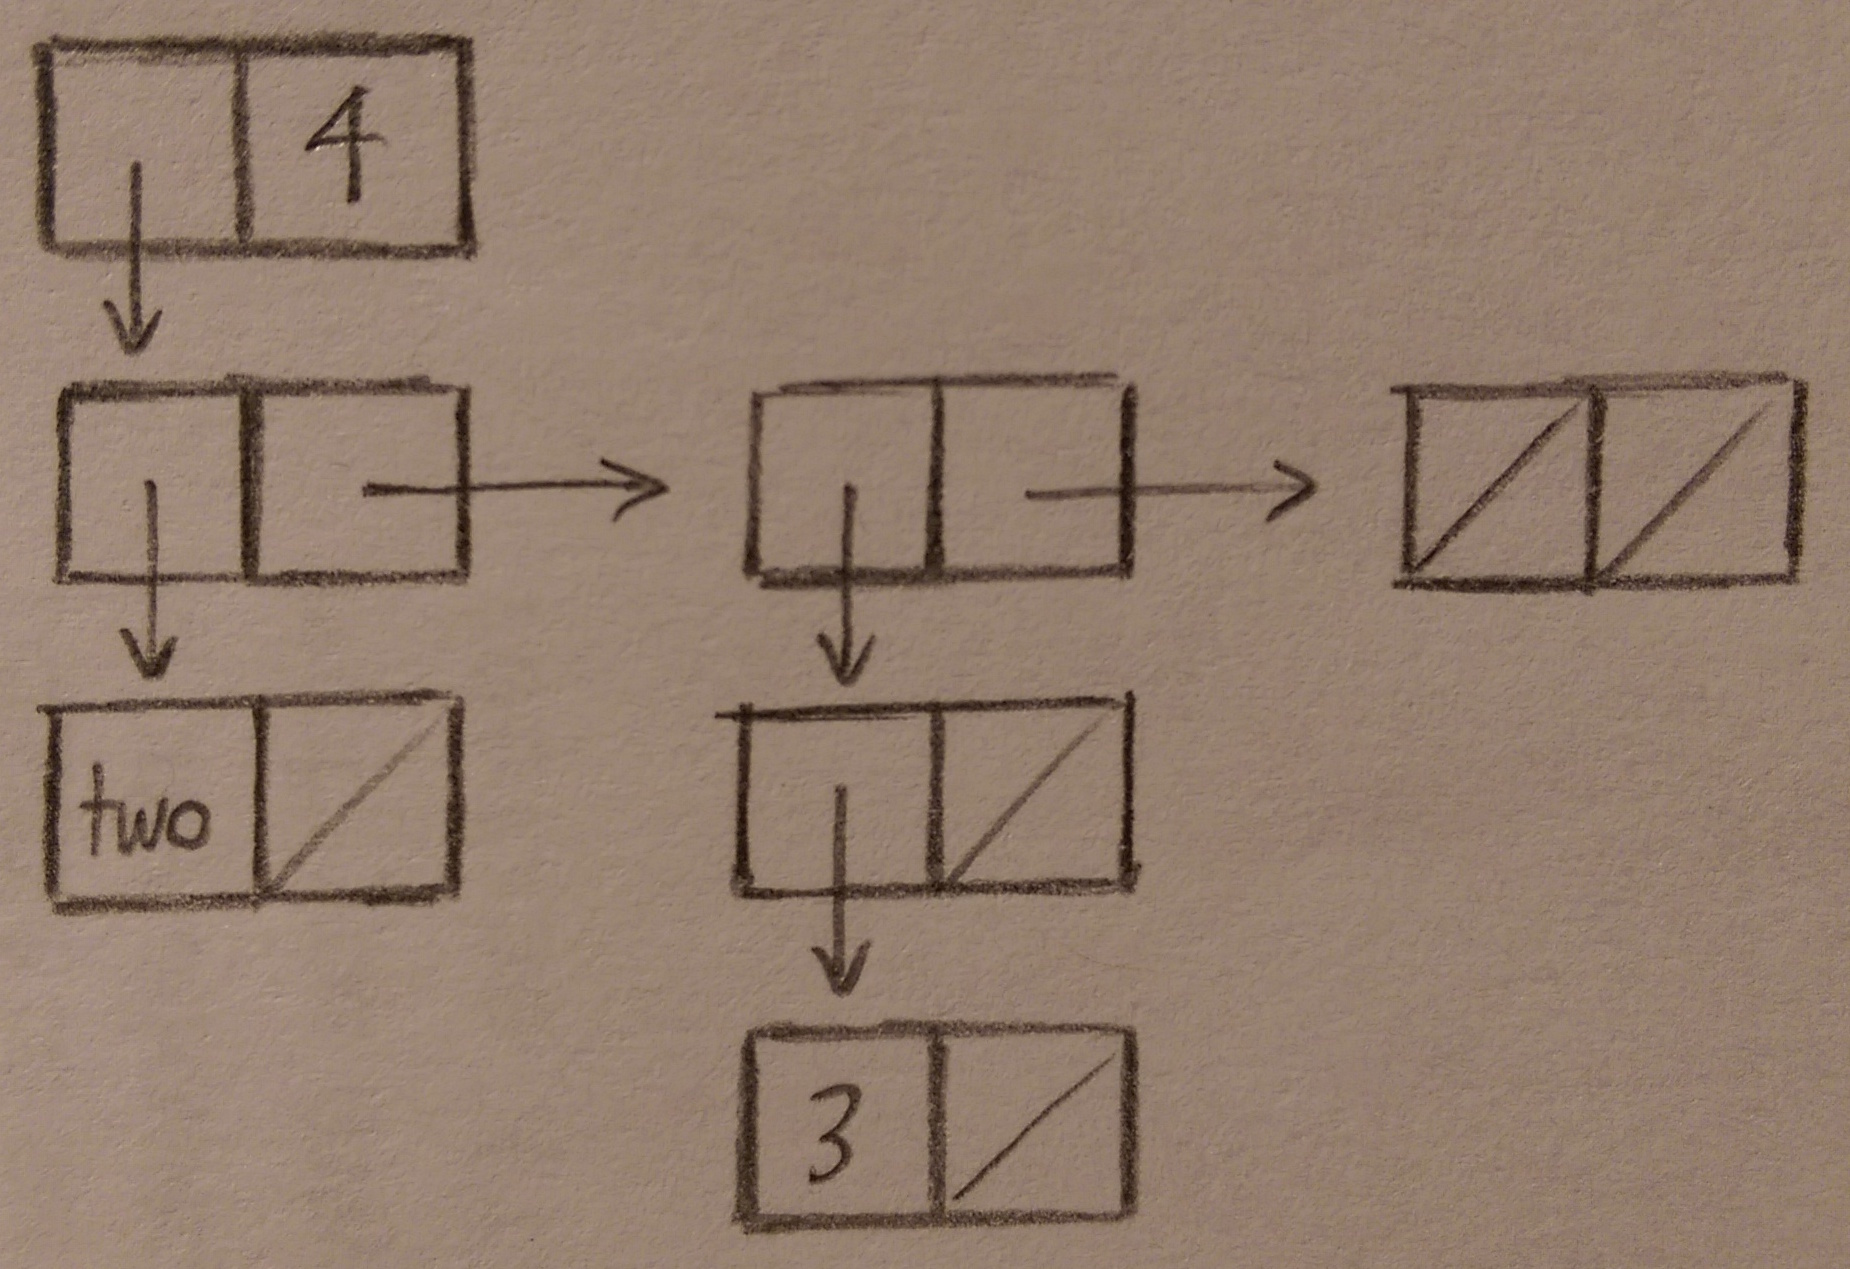
\includegraphics[scale=0.09]{3b_sol}*>

scm> (cons 2 '(list nil))
<*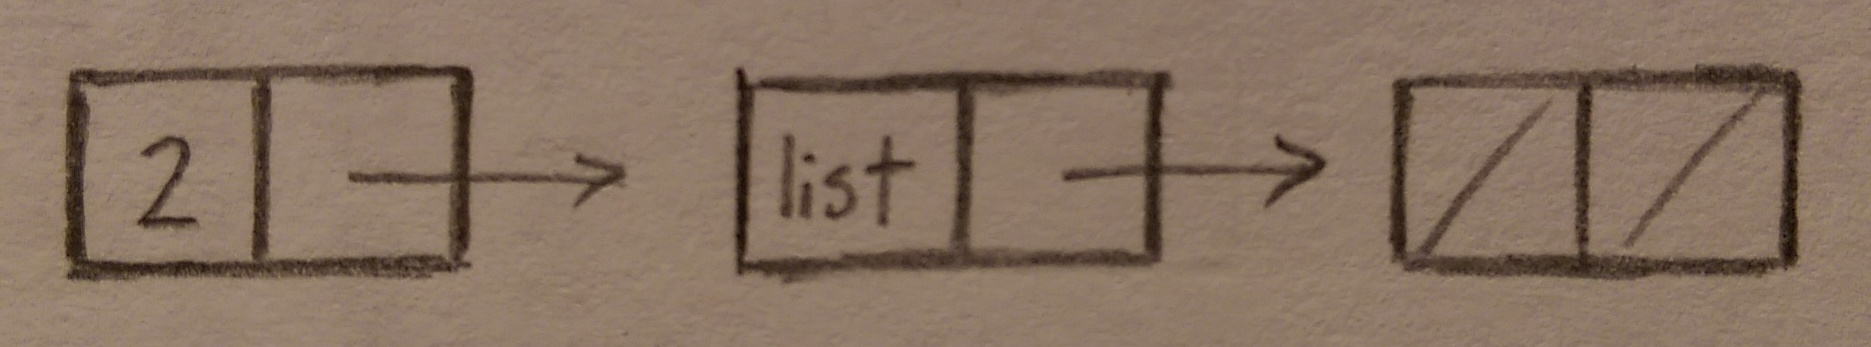
\includegraphics[scale=0.09]{3c_sol}*>

scm> (list (append '(2) '(3) nil) 4)
<*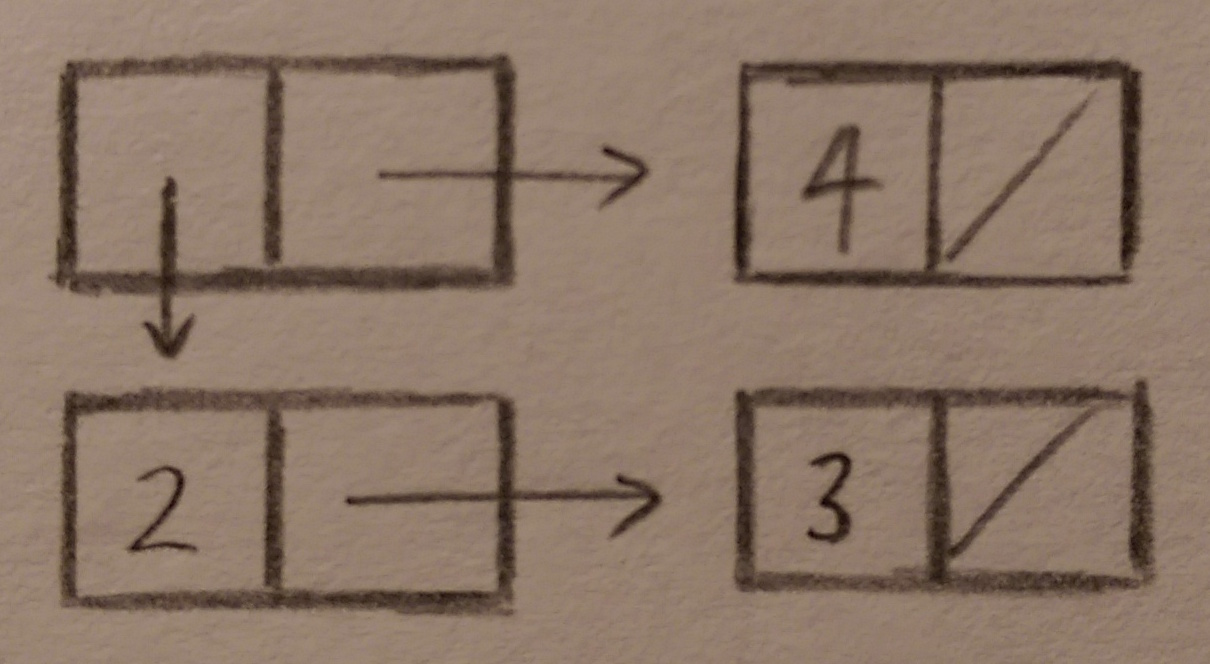
\includegraphics[scale=0.09]{3d_sol}*>

scm> '(2 . (3 . (4)))
<*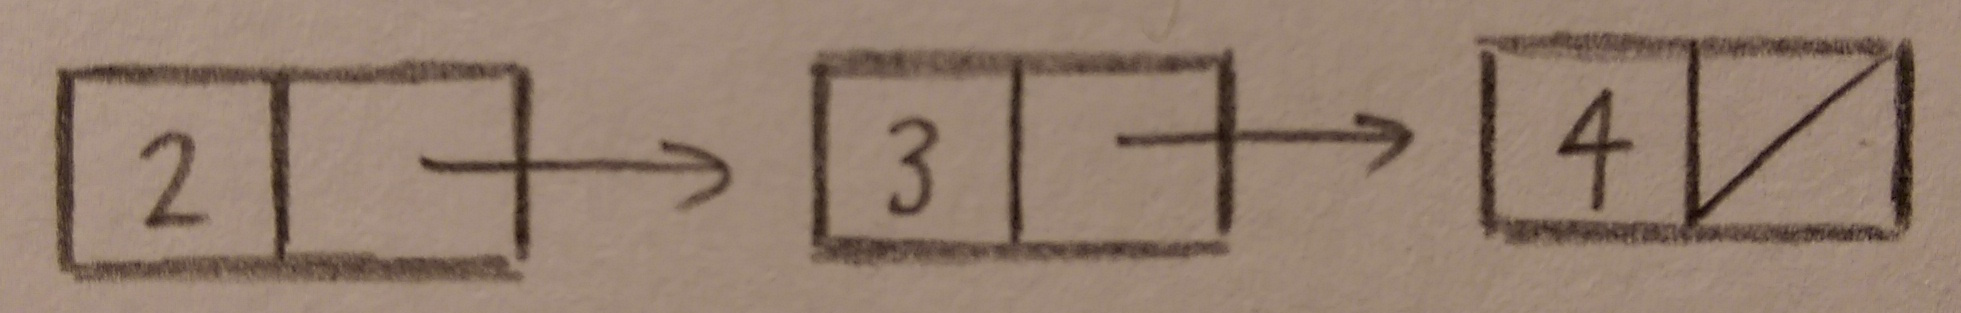
\includegraphics[scale=0.09]{3e_sol}*>
\end{lstlisting}

%%% Q4: Last One %%%
\q{4}{Last One}

Write a function \lstinline{take} that takes in a list \lstinline{s} and a positive number \lstinline{n}, and
returns a list \lstinline{t} such that \lstinline{(car t)} is the first \lstinline{n} elements of \lstinline{s} and \lstinline{(cdr t)}
is the remaining elements of \lstinline{s}. If \lstinline{n} is greater than the length of \lstinline{s}, \lstinline{(car t)} should be \lstinline{s} and \lstinline{(cdr t)} should be \lstinline{nil}.

\begin{lstlisting}
(define (take s n)
  <*\solution{(cond ((= n 0) (cons nil s))}*>
       <*\solution{((null? s) (cons s nil))}*>
       <*\solution{(else (let ((rec (take (cdr s) (- n 1))))}*>
            <*\solution{(cons (cons (car s) (car rec)) (cdr rec))))}*>
  <*\solution{)}*>
)
\end{lstlisting}

Example usage:

\begin{lstlisting}
scm> (define a (take '(1 2 3) 2))
scm> (car a)
(1 2)
scm> (cdr a)
(3)
scm> (define b (take '(1 2 3) 4)) ; n > (length s)
scm> (car b)
(1 2 3)
scm> (cdr b)
()
\end{lstlisting}

\end{enumerate}
\end{document}
